\section{Chiplet互联技术}

芯片能否成功跟上摩尔定律,很大程度上取决于芯片在一个封装中放置的距离,以确保它们之间快速、高带宽的电连接;就像单片 SoC 中的功能一样。Chiplet 互联技术是实现多 Die 系统(Multi-Die System)的关键,它定义了封装内不同芯片裸片(Die)之间如何进行高速、低延迟、高能效的数据通信。

3D 系统集成领域正在出现两个主要的行业方向:通过公共基板(也称为中介层)并排连接芯片的 2.5D 芯片集成和 3D-SoC,其中芯片彼此堆叠。Chiplets 提供了一个模块化系统,它将来自不同供应商和技术节点的独立芯片组合在一起,而不是将所有功能设计到一个单片系统中,下面将依次介绍不同的封装方式及与之对应的互联方式。

\subsection{2D MCM封装互联}

MCM(multi chip module, 多芯片组件) 封装, 即基板平面方向
集成多个芯片或芯粒, 是比较成熟的先进封装技术, 一般是指通过引
线键合 (bonding) 或/和倒装芯片 (flip chip) 技术实现芯粒和有机
基板 (substrate, 以下简称基板) 连通, 最终芯粒之间通过基板实现
互连。因为引线键合只能在芯粒四周出连线, 互连密度低, 信号线
长, 不利于高速信号互连, 所以在chiplet中更多应用基于高密度基板
的倒装芯片MCM, 基板上的走线宽度/间距可达$9/12\mu\text{m}$, 芯粒到芯
粒的间隙可以到 $1\text{ mm}$, 保证了芯粒互连信号质量, 同时有利于缩小
封装尺寸, 控制封装成本。采用MCM封装技术的典型芯片是AMD公
司基于Zen架构的服务器和台式电脑处理器芯片, 国内寒武纪公司云
端训练芯片思元$370$也采用MCM封装形式完成 $2$ 个芯粒的互连。

\subsection{2.3D封装互联}

2.3D 封装是指在一个有机转接板上实现芯粒之间的互连, 然后再 和基板相连, 如图 4(a) 所示。它将高密度有机转接板和低密度基板 分开制造, 便于提高基板良率和降低封装成本。 2.3D 封装中有机转接 板很薄, 由于没有玻纤等增强材料, 刚度很低, 所以翘曲 (warpage) 控制是个难点。

\begin{figure}[htbp]
	\centering
	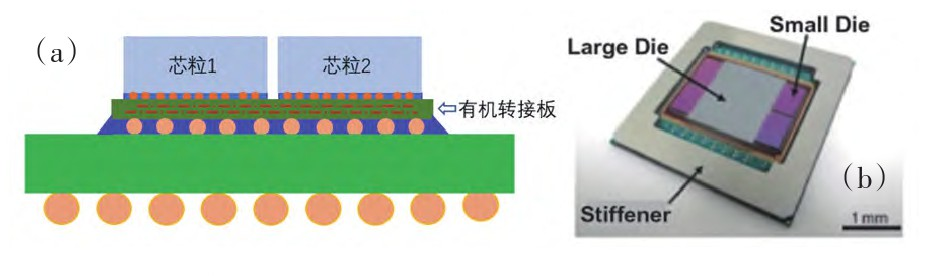
\includegraphics[width=0.6\textwidth]{img/3-2.jpg} % 图片文件名,不需要加扩展名
	\caption{$ \ 2.3\text{D}$ 封装概念图 $(\text{a})$ 及采用 $2.3\text{D}$ 封装的 $\text{Cisco}$ 公司芯片 $(\text{b})$ \cite{Miki2019Development}}
	\label{fig:example}
\end{figure}

目前有报道 Cisco 公司一款芯片已成功运用该技术, 产品线宽/间 距为 6/6μm, 集成 5 个芯粒, 如图 4(b) 
所示。国内目前已有公司 在开发双基板封装, 理念和 2.3D 封装类似, 只不过其基板互连密度没 有 2.3D 有机转接板高。

\subsection{以华为昇腾为例的Chiplet互联方式}

\begin{figure}[htbp]
	\centering
	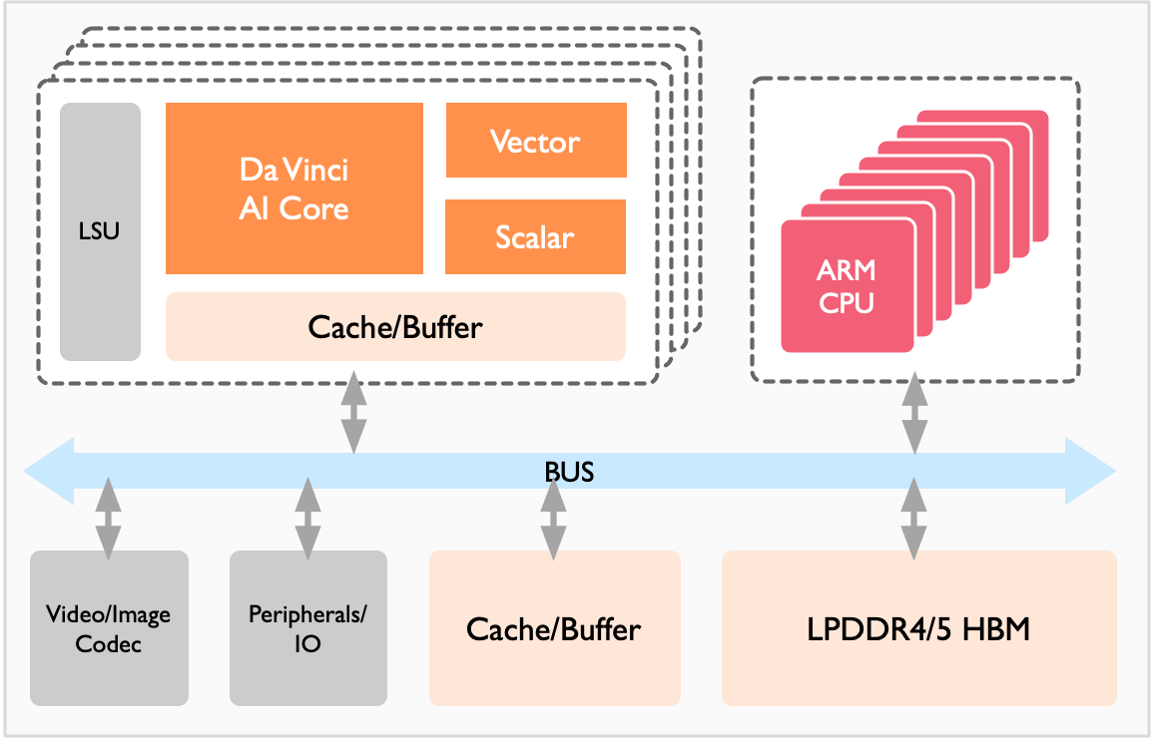
\includegraphics[width=0.6\textwidth]{img/5.png} % 图片文件名,不需要加扩展名
	\caption{基于 DaVinci AI 技术架构 \cite{CnblBlog2025}}
	\label{fig:example}
\end{figure}


昇腾 AI 处理器本质上是一个片上系统(System on Chip,SoC),主要可以应用在和图像、视频、语音、文字处理相关的应用场景。下图是早期昇腾其处理器的逻辑架构,其主要的架构组成部件包括特制的计算单元、大容量的存储单元和相应的控制单元。无论是训练还是推理的芯片以及上层的硬件型号,基于 DaVinci AI 技术架构如图5所示。

\begin{figure}[htbp]
	\centering
	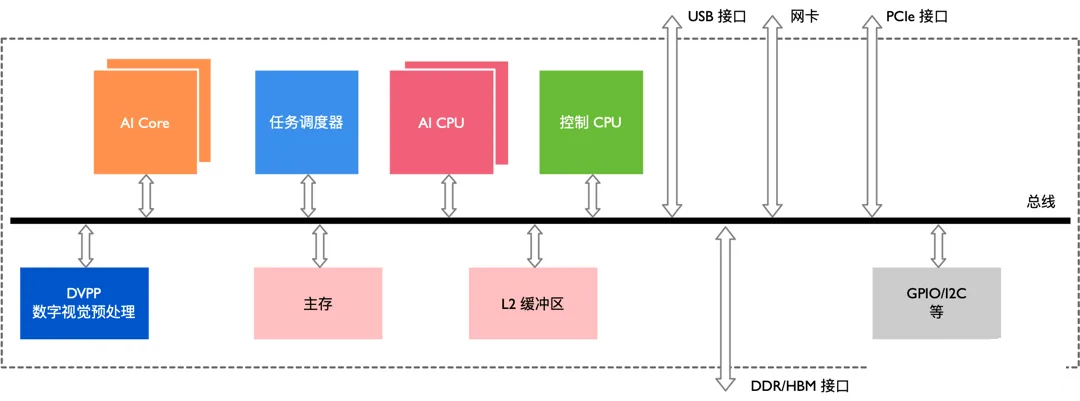
\includegraphics[width=0.8\textwidth]{img/6.png} % 图片文件名,不需要加扩展名
	\caption{ PCIe 总线接口传输总线用以实现数据互换 }
	\label{fig:example}
\end{figure}

该处理器大致可以划为:芯片系统控制 CPU(Control CPU),AI 计算引擎(包括 AI Core 和 AI CPU),多层级的片上系统缓存(Cache)或缓冲区(Buffer),数字视觉预处理模块(Digital Vision Pre-Processing,DVPP)等。芯片可以采用 LPDDR4 高速主存控制器接口,价格较低。目前主流 SoC 芯片的主存一般由 DDR(Double Data Rate)或 HBM(High Bandwidth Memory)构成,用来存放大量的数据。HBM 相对于 DDR 存储带宽较高,是行业的发展方向。其它通用的外设接口模块包括 USB、磁盘、网卡、GPIO、I2C 和电源管理接口等。

\subsection{昇腾 910的相关架构}

昇腾 910 处理器的目标场景是云端的推理和训练,其架构如图所示,包含 Davinci Core、DVPP、HBM、DDR4 等组件。

\begin{figure}[htbp]
	\centering
	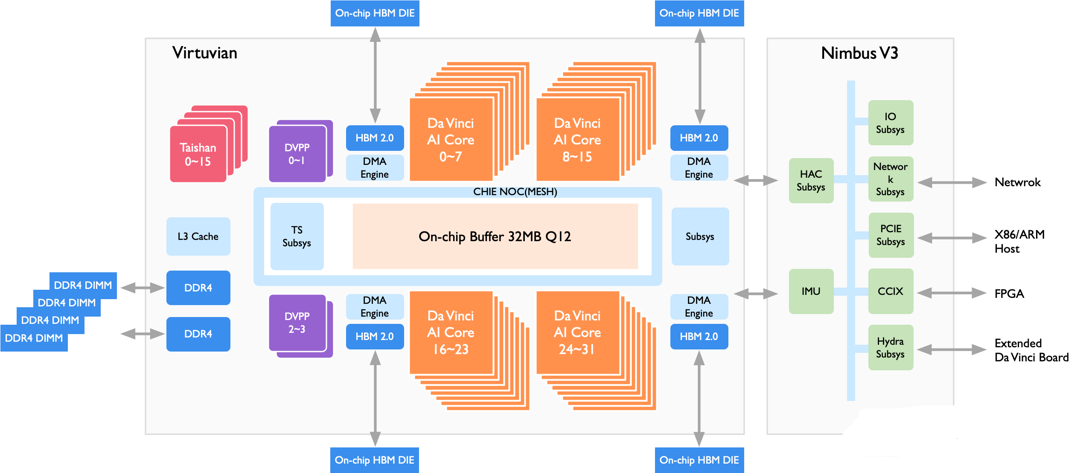
\includegraphics[width=0.8\textwidth]{img/7.png} % 图片文件名,不需要加扩展名
	\caption{昇腾 910 处理器的相关架构 }
	\label{fig:example}
\end{figure}

昇腾 910 处理器采用了芯粒(chiplet)技术,包含六个 die: 1 个计算芯粒(包含 32 个 Davinci Core、16 个 CPU Core 和 4 个 DVDP),1 个 IO 芯粒,和 4 个 HBM 芯粒(总计 1.2TB/s 带宽)。

该架构利用 AI Core 来加速通用卷积计算,总线接口从核外 L2 缓冲区或者直接从内存中读取卷积程序编译后的指令,送入指令缓存中,完成指令预取等操作,等待标量指令处理队列进行译码。如果标量指令处理队列当前无正在执行的指令,就会即刻读入指令缓存中的指令,并进行地址和参数配置,之后再由指令发射模块按照指令类型分别送入相应的指令队列进行执行。在卷积计算中首先发射的指令是数据搬运指令,该指令会被发送到存储转换队列中,再最终转发到存储转换单元中。


